\chapter{Trigonometry}
\begin{Definition}[sine and cosine]
The \emph{cosine} and \emph{sine} of an angle $\theta$ are the
$x$ and $y$ coordinate of the following point on a unit circle:
\begin{center}
  \begin{tikzpicture}
    \draw[-latex,thick] (-3,0) -- (3,0);
    \draw[-latex,thick] (0,-3) -- (0,3);
    \draw (0,0) circle (2);

    \draw (0,0) -- (60:3);
    \draw (0:.5) arc [start angle=0,end angle=60,radius=0.5] node[midway,anchor=south west,font=\tiny,inner sep=1mm] {$\theta$};

    \draw[dotted] let \p1=(60:2) in (\p1) -- (\x1,0) node[anchor=north,font=\tiny] {$\cos \theta$};
    \draw[dotted] let \p1=(60:2) in (\p1) -- (0,\y1) node[anchor=east,font=\tiny] {$\sin \theta$};
  \end{tikzpicture}
\end{center}
\end{Definition}

Drawing both these trigonometric functions yields the following graph:
\begin{center}
  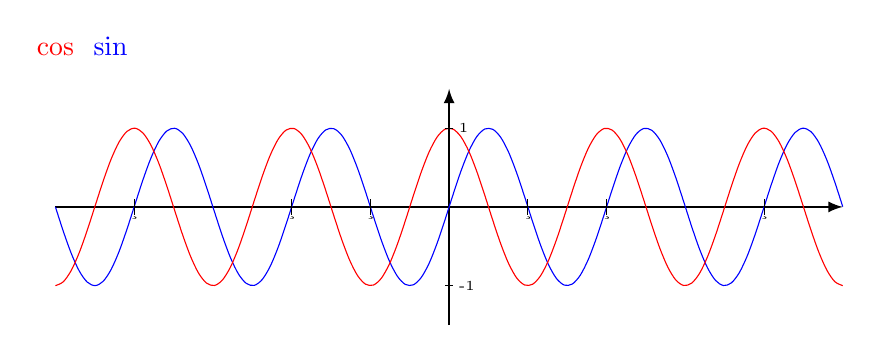
\begin{tikzpicture}
    \draw[-latex,thick] (-5,0) -- (5,0);
    \draw[-latex,thick] (0,-1.5) -- (0,1.5);

    \draw[blue,domain=-5:5,smooth,samples=100] plot (\x,{sin(180 * \x)});
    \draw[red,domain=-5:5,smooth,samples=100] plot (\x,{cos(180 * \x)});

    \foreach \x in {-4,-2,-1,1,2,4} {
      \tikzmath{
        real \c;
        \c = int(\x * 180);
      }
      \draw (\x,-0.1) -- (\x,0.1);
      \node[anchor=north,font=\tiny] at (\x,0) {\c\degrees};
    }

    \draw (-0.05,1) -- (0.05,1);
    \draw (-0.05,-1) -- (0.05,-1);
    \node[anchor=west,font=\tiny] at (0,1) {1};
    \node[anchor=west,font=\tiny] at (0,-1) {-1};

    \node (cos) at (-5,2) {\color{red}$\cos$};
    \node[anchor=base west] (sin) at (cos.base east) {\color{blue}$\sin$};
  \end{tikzpicture}
\end{center}

Some noteworthy values are
\[
  \begin{array}{ccc}
    \theta & \cos\theta & \sin\theta \\
    \toprule
    0\degrees & 1 & 0 \\
    90\degrees & 0 & 1 \\
    180\degrees & -1 & 0 \\
    270\degrees & 0 & -1 \\
  \end{array}
\]

\begin{theorem} \label{thm:sin-cos-relation}
For any angle $\theta$,
\[
  \cos(\theta)^2 + \sin(\theta)^2 = 1
\]
\end{theorem}

%%% Local Variables:
%%% mode: latex
%%% TeX-master: "reference"
%%% End:
